\chapter{ASMIS Use Cases}

\begin{figure}[h!]
\centering
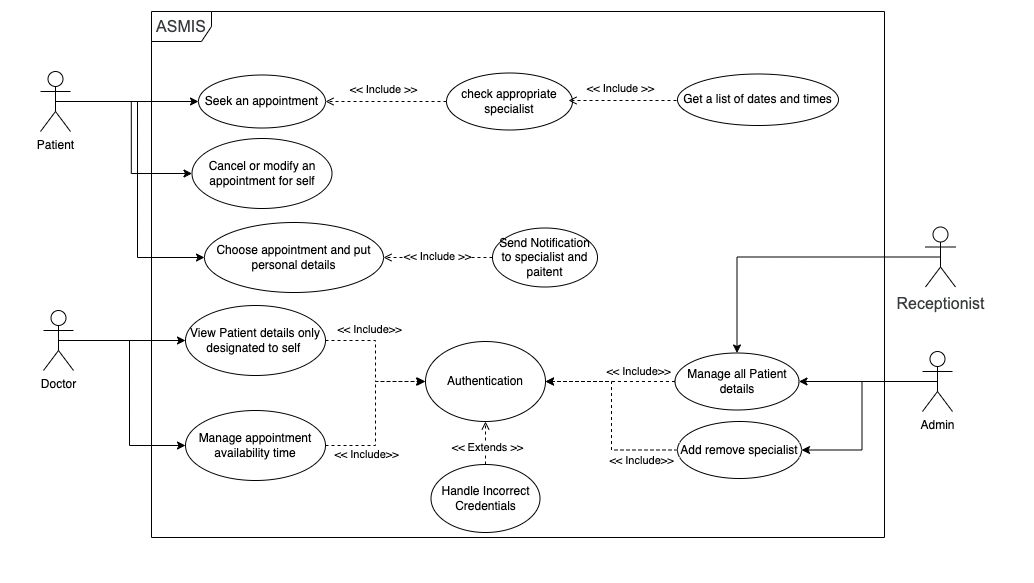
\includegraphics[width=\textwidth]{pics/usecase.png}
\caption{Use case diagram for ASMIS}\label{fig:usecase}
\end{figure}

\section{Overview}
The use case is a very insightful UML diagram that allows us to capture, identify, and analyze the system under development. The diagram analyzes the system by dividing the actions possible using different actors \citep[p.~64]{jacobson2021unified}. In this case, the use case shows us the possible paths to be available for the ASMIS application and could be the base to apply an abuse case threat modeling \citep [p.~59]{usecase_abuse_case}.


\section{Analyzing Use Case}
Figure \ref{fig:usecase} depicts a use case diagram for the ASMIS system for the Queens medical center. This application will provide a platform for the patient and the clinic staff to manage and operate the scheduling efficiently and swiftly. \newline\newline
The application consists of four main actors the patient, the doctor/specialist, the receptionist, and the admin. The patient can seek an appointment using the application without logging in by inputting the desired health-related issue. After this step, the application determines the appropriate specialists for the patient and presents the list of available appointments. Lastly, the patient chooses the date and the specialist with personal data, including name, address, email, and phone number, which would send a confirmation email.\newline\newline
From the use case diagram, one can see that specialists and admin can manage the appointment schedules and also check the patient who booked an appointment. The main difference between the admin, the receptionist, and the specialist is the right to see data. The specialist can only see the patient data assigned to own, but admins and receptionists can manage all patient data. Similarly, the other actors, the specialist, the receptionist, and the admin, must authenticate to carry out any actions. Additionally, the admins can add and remove specialists and receptionists in the system and allocate them privileges. 